% !TEX root = ../main.tex
\section{Problem analysis}

\begin{frame}{Problem analysis}
  \begin{block}{Objective}
    Detect whether the input speech is one of 35 keywords or not.
  \end{block}
  \begin{figure}
    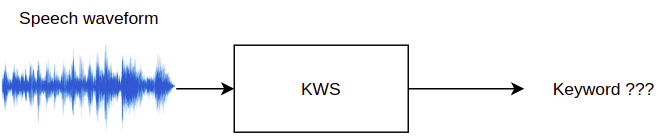
\includegraphics[width=\textwidth]{figure/KWS.png}
    \caption{Keyword Spotting System structure}
  \end{figure}
\end{frame}

\begin{frame}{Problem analysis}
  \begin{columns}
    \begin{column}{0.3\textwidth}
      \begin{block}{Model was used:}
        - Based on M5 model \autocite{7952190}

        - The struture of M5 is described in figure \ref{fig:m5-model}
      \end{block}
    \end{column}

    \begin{column}{0.6\textwidth}
      \begin{figure}
        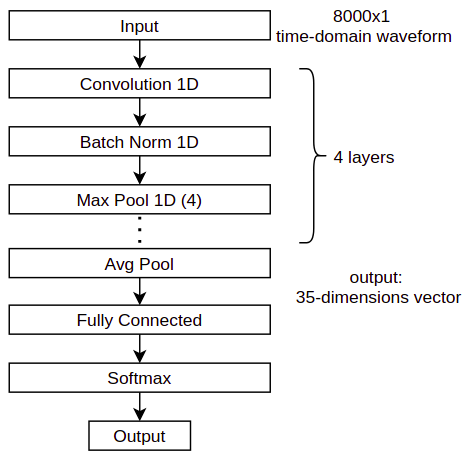
\includegraphics[width=0.8\textwidth]{figure/m5model.png}
        \caption{M5 structure}
        \label{fig:m5-model}
      \end{figure}
    \end{column}
  \end{columns}
\end{frame}

\begin{frame}{Problem analysis}
\begin{columns}
  \begin{column}{0.7\textwidth}
    \begin{block}{Dataset}
    - \textbf{Speech Commands} dataset of Cornell University

    - Number of keywords: 35

    - Number of sample file: 105,835

    - Sample rate: 16000 Hz
    \end{block}  

    \begin{block}{Data division}
      - Size of train data: 105,829 files

      - Size of test data: 11,005 files
    \end{block}
  \end{column}
  
  \begin{column}{0.3\textwidth}
    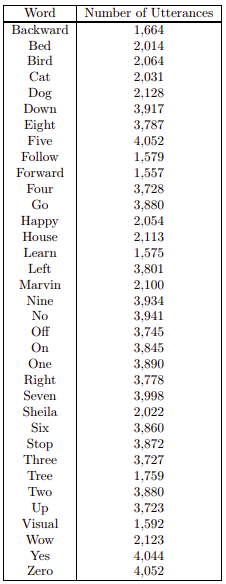
\includegraphics[width=0.7\textwidth]{figure/speech-command-info.png}
  \end{column}
\end{columns}
\end{frame}

